\documentclass{beamer}
\usepackage{caption}
\usepackage[utf8]{inputenc}
\usepackage[T1]{fontenc}


% Pour quel partie chaque personne parle :
% Mise en contexte -> Vital
% Technologies utilisées -> Vital
% Différentes stratégies pour un rendu 3D :
%   Approche historique -> Matthieu
%   Explication de DDA  -> Matthieu
%   Approche moderne -> Matthieu
% Construction de mur -> Vital
% Les collisions -> Elian
% Les portails -> Elian
% Les renders -> Matthieu
% Conclusion -> Elian


\usetheme{Boadilla}

\begin{document}

% Définition de la mise en page du pied de page avec un espacement réduit
\setbeamertemplate{footline}{%
  \leavevmode%
  \hbox{\begin{beamercolorbox}[wd=\paperwidth,ht=2.25ex,dp=1ex,center]{author in head/foot}%
    \usebeamerfont{author in head/foot}\insertshortauthor\hspace*{2em}
    \insertshorttitle\hspace*{2em}\insertframenumber{} / \inserttotalframenumber
  \end{beamercolorbox}}%
  \vskip0pt%
}

\title{Présentation du projet Portal 0.0}
\author[BADSTÜBER E. BIDAULT M. FOCHEUX V.]{BADSTÜBER Elian BIDAULT Matthieu FOCHEUX Vital \\
                                                Licence 3 Informatique}
\date{Mars 2024}

\setcounter{framenumber}{0}
% \setbeamertemplate{page number in head/foot}{}

{
\setbeamertemplate{footline}{}
\begin{frame}
    \titlepage
    
    \vfill % Insertion d'un espace vertical flexible pour pousser le texte en bas
    \begin{columns}
        \column{0.3\textwidth}
        \centering
        
\includegraphics[width=\textwidth]{images/logo-UFR-ST.jpg} 
    
        \column{0.4\textwidth}
        \begin{flushright}
            \small Tuteur : Julien BERNARD
        \end{flushright}    
    \end{columns}
\end{frame}
}

\setcounter{framenumber}{0}
\setbeamertemplate{page number in head/foot}[totalframenumber]

\begin{frame}
    \frametitle{Table des matières}
    \tableofcontents
\end{frame}

\section{Mise en contexte}

\begin{frame}
    \frametitle{Mise en contexte}
    \begin{block}{}
        % Portal 0.0 est un jeu vidéo qui reprends les principes techniques 
        % de plusieurs jeux vidéos connus.
        \begin{itemize}
            \item Portal 0.0 $\rightarrow $ principes techniques de plusieurs jeux vidéos connus
        \end{itemize}
    \end{block}

    \begin{block}{Technique graphique}
        \begin{itemize}
            \item Méthode raycasting
            \item Rendu 2.5D popularisé dans les années 90
            \item Principe de Wolfenstein3D (1992)
        \end{itemize}
        % L'utilisation de la méthode du raycasting, pour un rendu 2.5D qui a été 
        % popularisé dans le début des années 90.
    \end{block}

    \invisible{\begin{block}{Système de jeu}
        \begin{itemize}
            \item Résolution d'énigmes à l'aide de portails
            \item Téléportation lorsqu'on passe à travers
            \item Principe de Portal (2007)
        \end{itemize}
        % Le principe du jeu vidéo Portal (2007), où l'on doit résoudre des énigmes
        % à l'aide de portails, dans lesquels on se téléporte lorsqu'on passe à travers.
    \end{block}}
\end{frame}

\begin{frame}
    \label{sl: identical-numbers}
    \frametitle{Mise en contexte}
    \begin{block}{}
        % Portal 0.0 est un jeu vidéo qui reprends les principes techniques 
        % de plusieurs jeux vidéos connus.
        \begin{itemize}
            \item Portal 0.0 $\rightarrow $ principes techniques de plusieurs jeux vidéos connus
        \end{itemize}
    \end{block}

    \begin{block}{Technique graphique}
        \begin{itemize}
            \item Méthode raycasting
            \item Rendu 2.5D popularisé dans les années 90
            \item Principe de Wolfenstein3D (1992)
        \end{itemize}
        % L'utilisation de la méthode du raycasting, pour un rendu 2.5D qui a été 
        % popularisé dans le début des années 90.
    \end{block}

    \begin{block}{Système de jeu}
        \begin{itemize}
            \item Résolution d'énigmes à l'aide de portails
            \item Téléportation lorsqu'on passe à travers
            \item Principe de Portal (2007)
        \end{itemize}
        % Le principe du jeu vidéo Portal (2007), où l'on doit résoudre des énigmes
        % à l'aide de portails, dans lesquels on se téléporte lorsqu'on passe à travers.
    \end{block}
\end{frame}

\section{Technologies utilisées}

\begin{frame}
    \frametitle{Technologies utilisées}
    \begin{columns}
        \column{0.3\textwidth}
        \centering
        
\includegraphics[width=\textwidth]{images/cpp.png} 
    
        \column{0.4\textwidth}
        \centering
        
\includegraphics[width=\textwidth]{images/GF.png}
        \captionof{figure}{Gamedev Framework}

        \column{0.4\textwidth}
        \centering
        
\includegraphics[width=\textwidth]{images/github.png}
    \end{columns}
\end{frame}

\section{Détails du développement}
\subsection{Différentes stratégies pour un rendu 3D}

\begin{frame}
    \frametitle{Différentes stratégie pour un rendu 3D \\
                \small Approche historique}
    \begin{block}{Raycasting}
        \begin{itemize}
            \item Méthode de rendu graphique en 2.5D
            \item Illusion d'une perspective 3D à partir d'un environnement 2D
            \item Projection de rayons depuis la position du joueur
        \end{itemize}
    \end{block}
    \begin{block}{Optimisation}
        % Le raycasting est une méthode de rendu graphique utilisée pour créer 
        % une perspective 3D dans des environnements 2D. Ce rendu est réalisé
        % en projetant des rayons depuis la position du joueur à travser la scène
        % pour déterminer les intersections avec les murs. Pour l'optimisation,
        % l'algorithme DDA (Digital Differential Analyzer) est utilisé.
        Lancé des rayons avec DDA (Digital Differential Analyzer).
    \end{block}
\end{frame}

\begin{frame}
    \frametitle{Différentes stratégie pour un rendu 3D \\
                \small DDA}           
    \begin{block}{}
        \begin{itemize}
            \item Conçu pour la rasterisation de lignes
            \item Repose sur l'itération linéaire
            \item Employé pour déterminer où les rayons projetés intersectent avec les objets de l'environnement
        \end{itemize}
    \end{block}    
    \begin{figure}
        \centering
        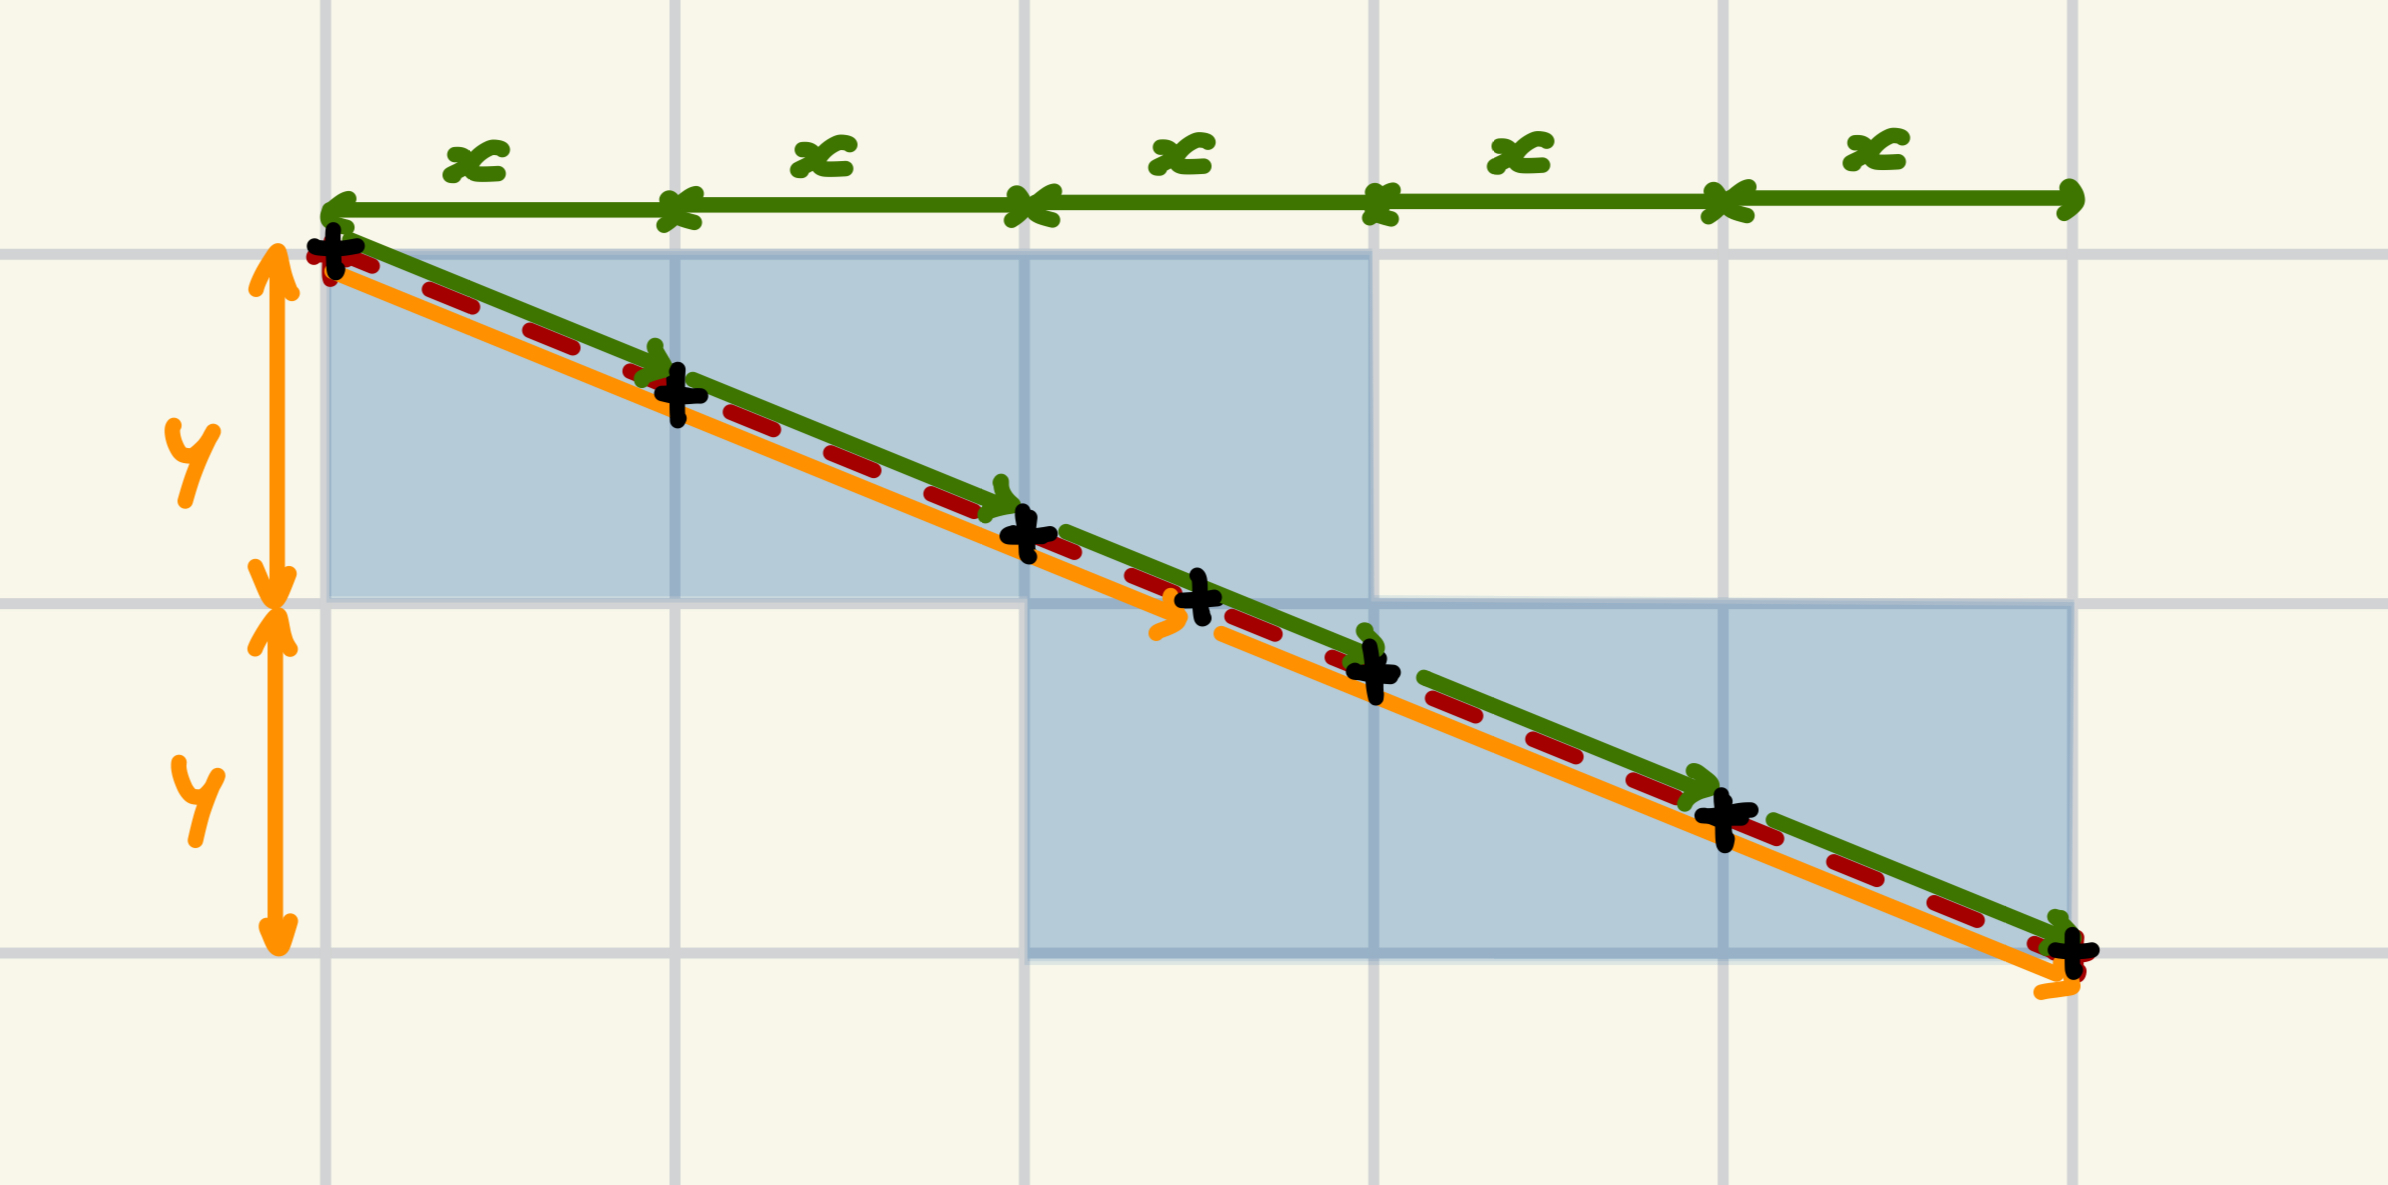
\includegraphics[width=0.7\textwidth]{images/DDA.jpg}
    \end{figure}
\end{frame}

\begin{frame}
    \frametitle{Différentes stratégie pour un rendu 3D \\
                \small DDA}           
    \begin{block}{}
        \center{Fonctionnement de DDA.}
    \end{block}    
    \begin{figure}
        \centering
        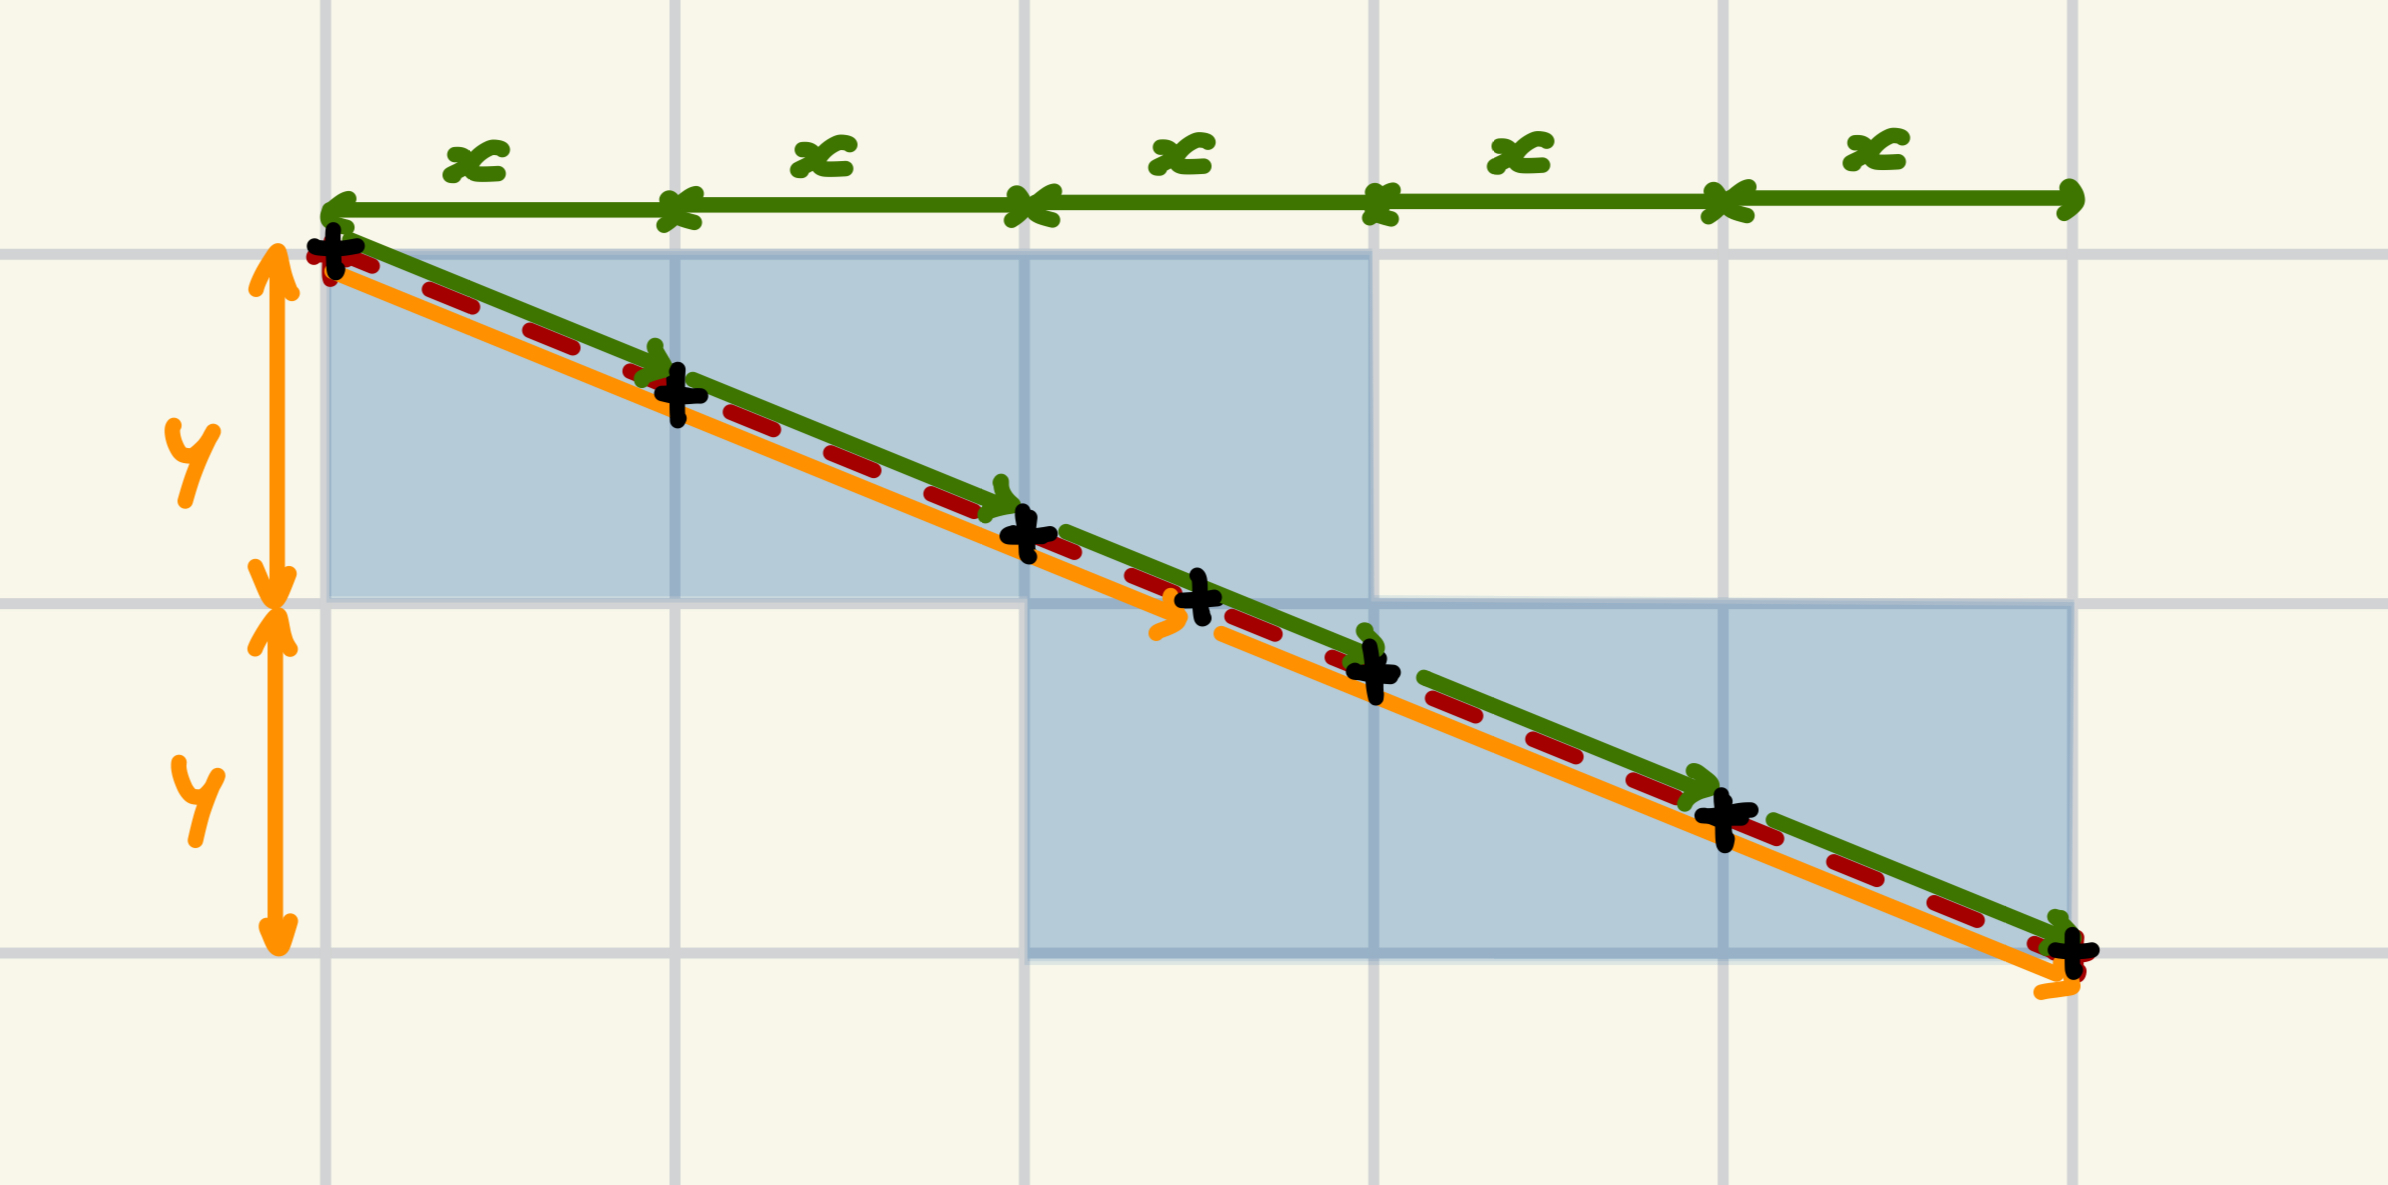
\includegraphics[width=0.7\textwidth]{images/DDA.jpg}
    \end{figure}
\end{frame}

% \begin{frame}
%     \frametitle{Différentes stratégie pour un rendu 3D \\
%                 \small DDA}           
%     \begin{block}{}
%         \begin{itemize}
%             \item Calcule l'emplacement correspondant sur l'autre axe en ajoutant un incrément constant
%             \item Utilisé pour trouver rapidement et précisément les intersections entre les rayons 
%             et les murs dans le raycasting
%         \end{itemize}
%         % L'algorithme DDA est historiquement conçu pour la rasterisation de 
%         % lignes, c'est-à-dire la conversion de lignes geometriques en ligne 
%         % visuelle composées de pixels alignés. Dans le contexte du raycasting, 
%         % DDA est employé pour déterminer où les rayons projetés à travers la 
%         % scène intersectent avec les objets de l'environnement, typiquement et 
%         % dans notre cas représenté par une grille de cellules. Le principe 
%         % fondamental de DDA repose sur l'itération linéaire. Plutôt que de 
%         % calculer chaque point le long d'une demie droite en utilisant des formules 
%         % de géométrie directe, ce qui pourrait être coûteux en termes de performances, 
%         % DDA avance par petits incr ́ements. Cela signifie que pour chaque
%         % pas sur l'axe le plus dominant (x ou y), DDA calcule l'emplacement 
%         % correspondant sur l'autre axe en ajoutant un incrément constant. 
%         % Cela se traduit par un parcours régulier et efficace le long de la 
%         % ligne en faisant des sauts à chaque intersection entre la demie 
%         % droite et la grille 2D. Dans le raycasting, DDA est utilisé pour 
%         % trouver rapidement et précisément les intersections entre les rayons 
%         % et les murs
%     \end{block}    
% \end{frame}

\begin{frame}
    \frametitle{Différentes stratégie pour un rendu 3D \\
                \small Approche moderne (Line Of Sight)}    
                
    
    \begin{block}{}
        \begin{itemize} 
            \item Envoyer un rayon pour chaque sommet de chaque mur
        \end{itemize}
%         Cette seconde approche s’approche des algorithme Line Of Sight et consiste
% a calculer la distance entre le joueur et chaque sommet de chaque mur.
% Pour ce faire on a pu recuperer l’algorithme DDA precedemment utilise
% pour le rendu des murs mais cette fois-ci en visant chaque sommets au lieu
% de viser chaque colonne de pixel. Cela permet theoriquement de reduire
% considerablement le nombre de calculs a effectuer.

    \end{block}    


    \begin{figure}
        \centering
        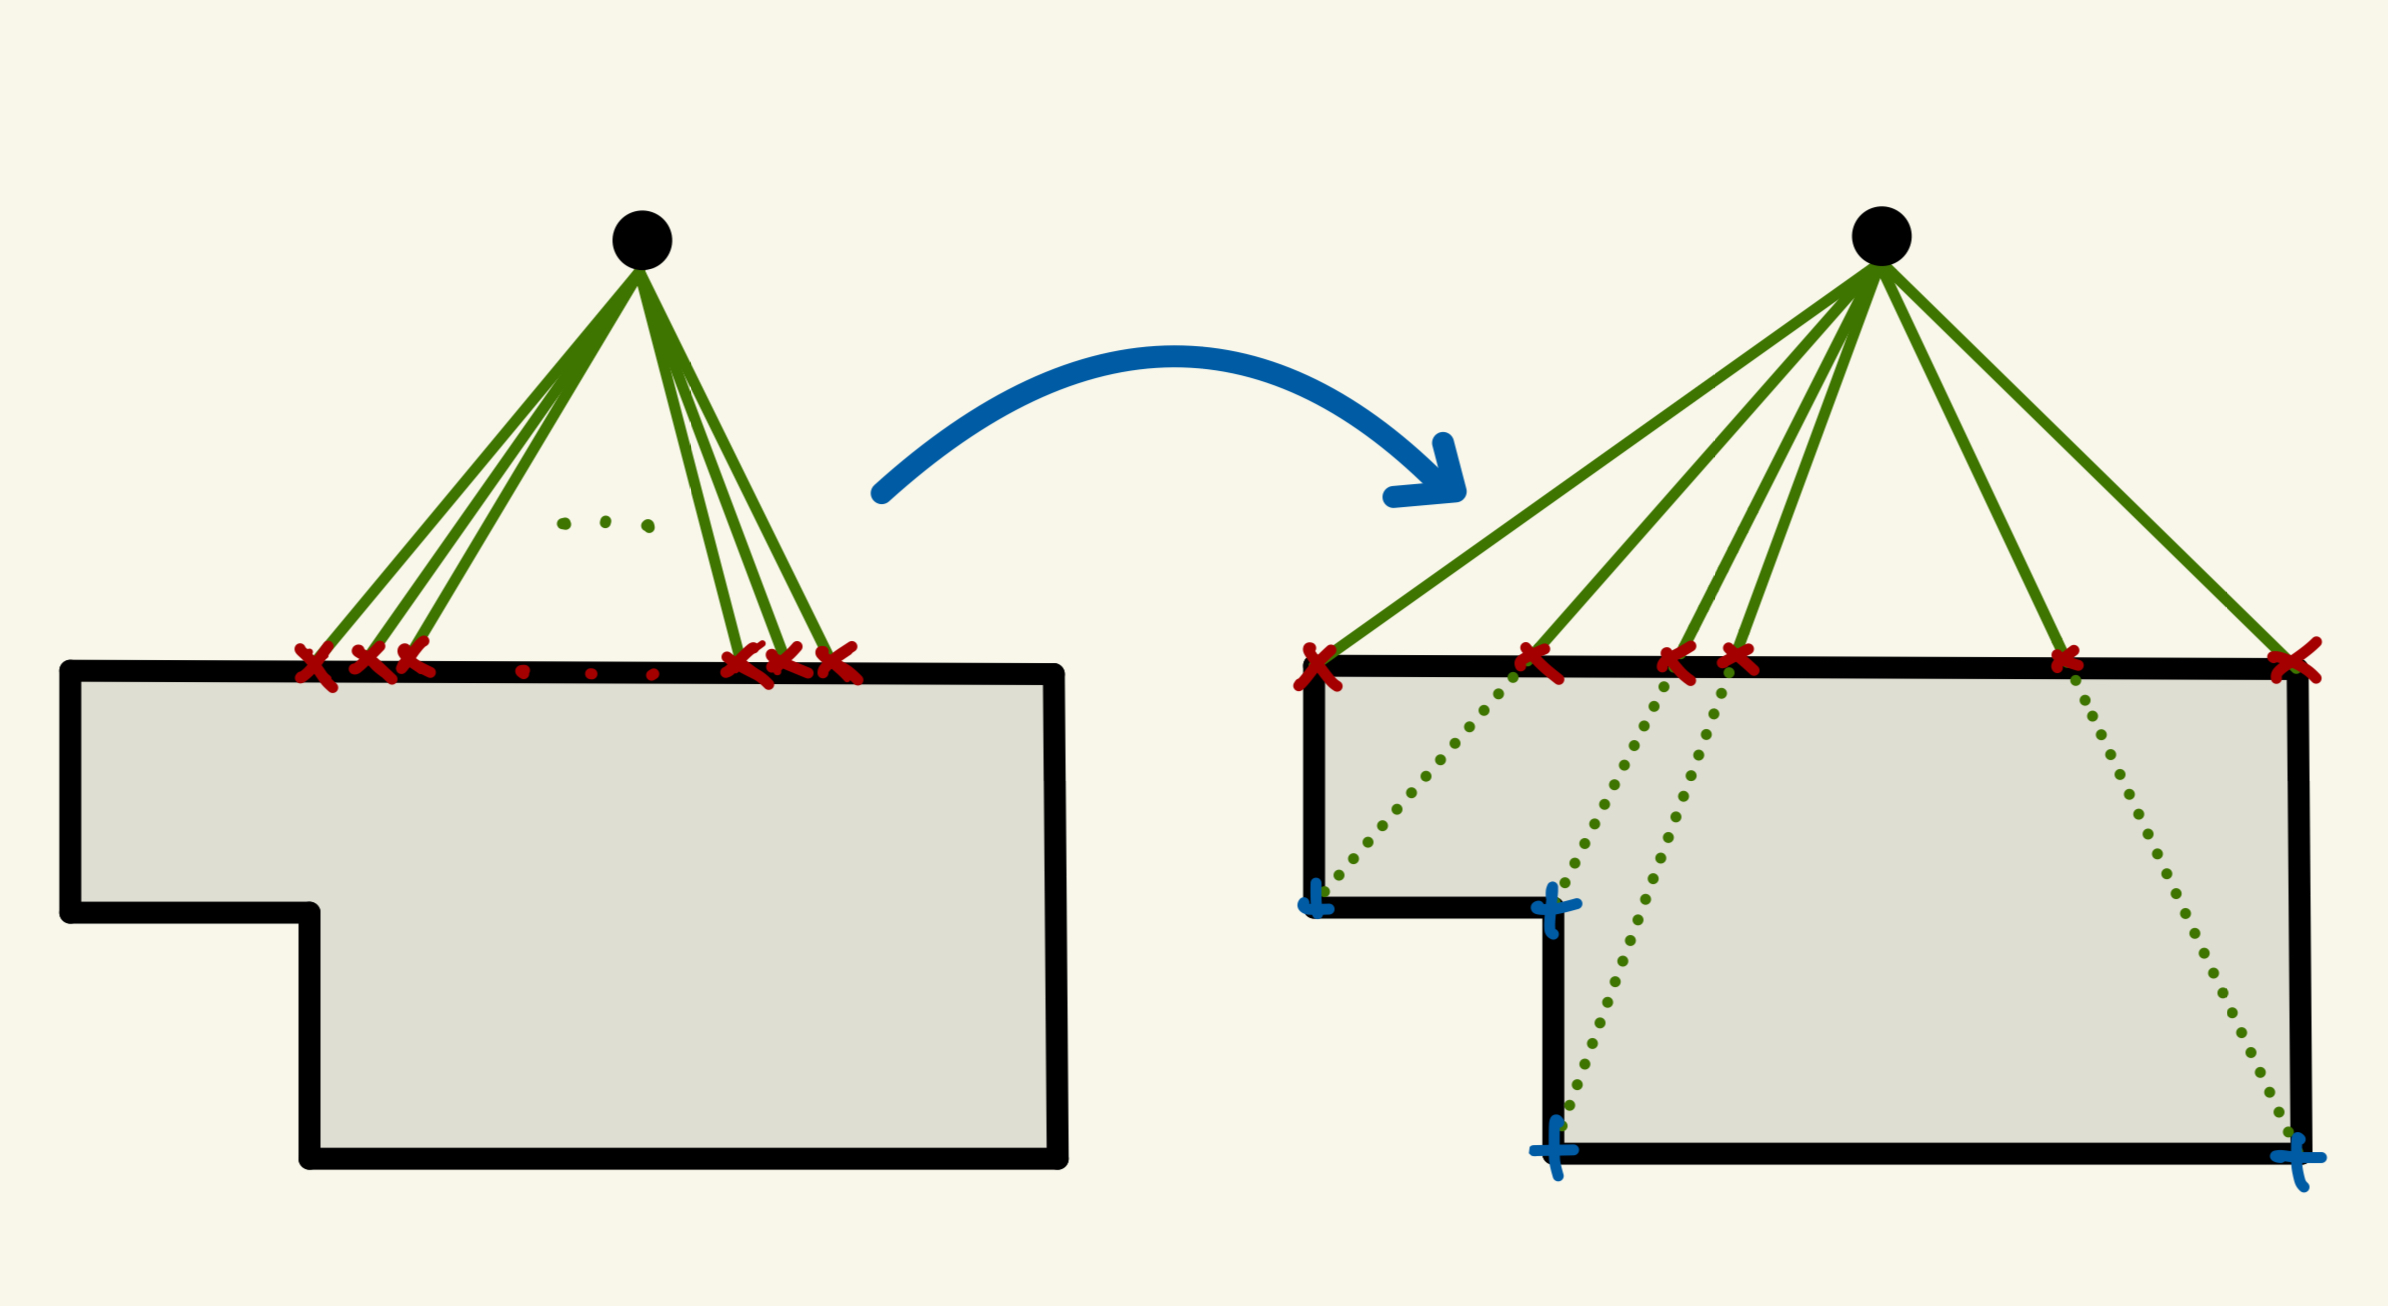
\includegraphics[width=0.8\textwidth]{images/comparaison-deux-methodes.jpeg}
    \end{figure}
\end{frame}

\subsection{Construction de mur}

\begin{frame}
    \frametitle{Construction de mur \\
                \small Sommets utiles}
    \begin{block}{}
        \begin{itemize}
            \item Boucle sur les coordonnées des cellules
            \item Vérification des sommets adjacents
        \end{itemize}
    \end{block}
    \begin{figure}
        \centering
        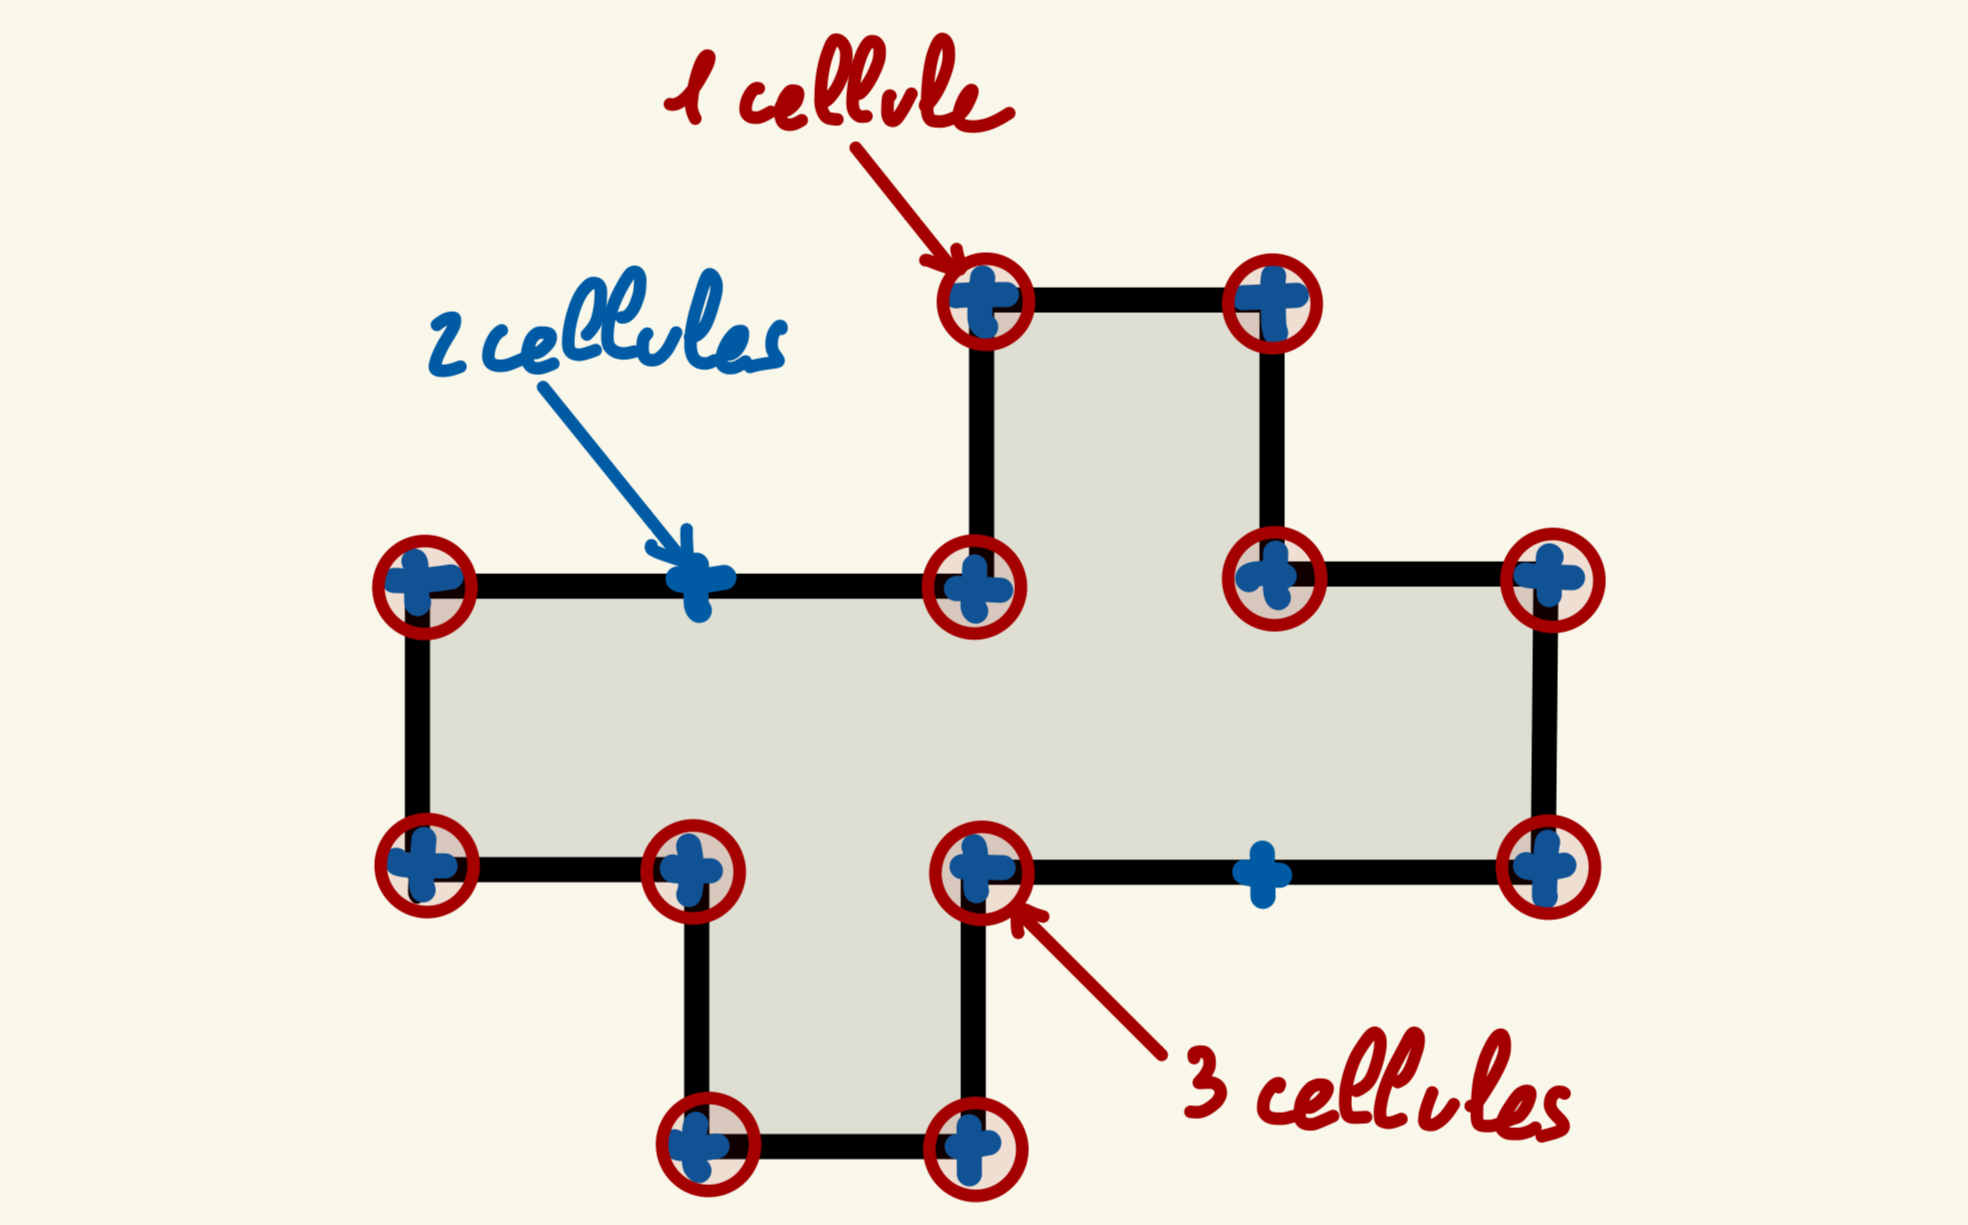
\includegraphics[width=0.7\textwidth]{images/sommets_utiles.jpg}
    \end{figure}
\end{frame}

\begin{frame}
    \frametitle{Construction de mur \\
                \small Trie des sommets}
    \begin{block}{}
        \begin{itemize}
            \item Boucle sur les sommets utiles
            \item Méthode : Droit > Bas > Gauche > Haut
        \end{itemize}
    \end{block}
    \begin{figure}
        \centering
        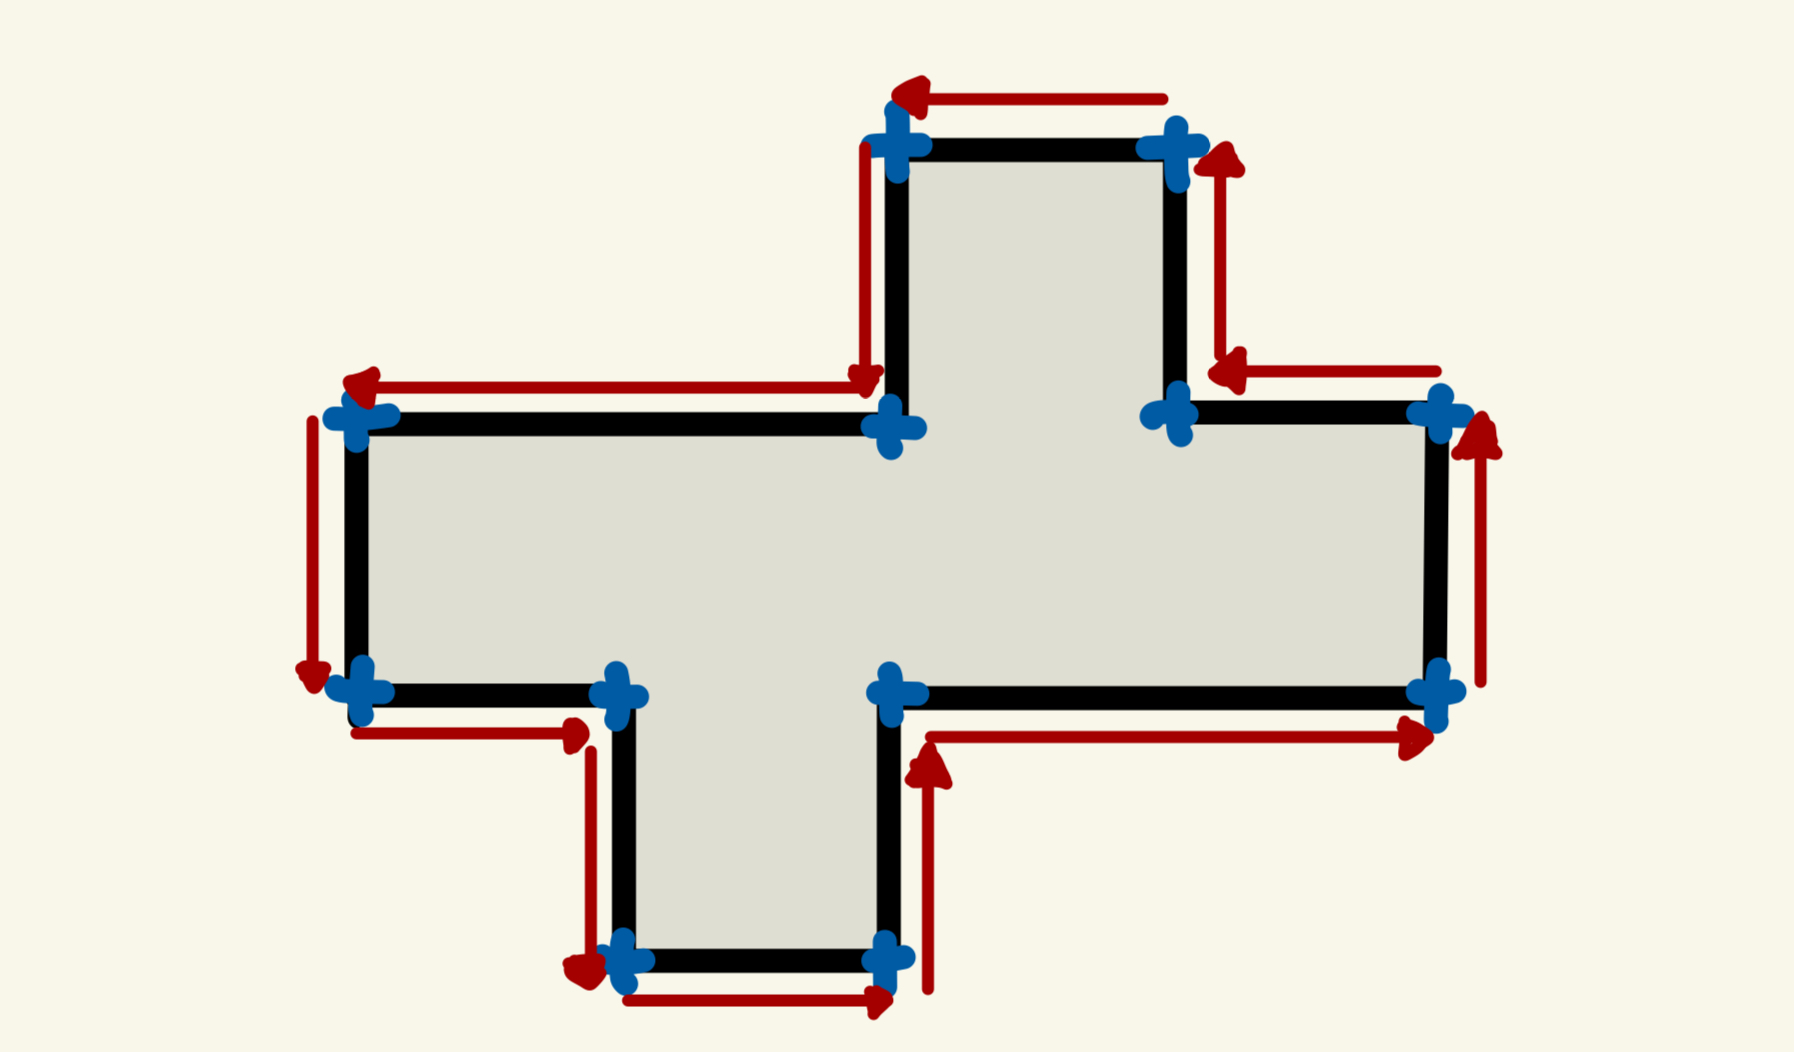
\includegraphics[width=0.7\textwidth]{images/tri_sommet.jpg}
    \end{figure}
\end{frame}

\subsection{Les collisions}

\begin{frame}
    \frametitle{Les collisions}
    \begin{block}{}
        \begin{itemize}
            \item Utilisation de la fonction clamp
        \end{itemize}
    \end{block}
\end{frame}

\section{Spécifications}
\subsection{Les portails}

\begin{frame}
    \frametitle{Les portails \\
                \small La téléportation}
    \begin{block}{}
        
    \end{block}
    \begin{figure}
        \centering
        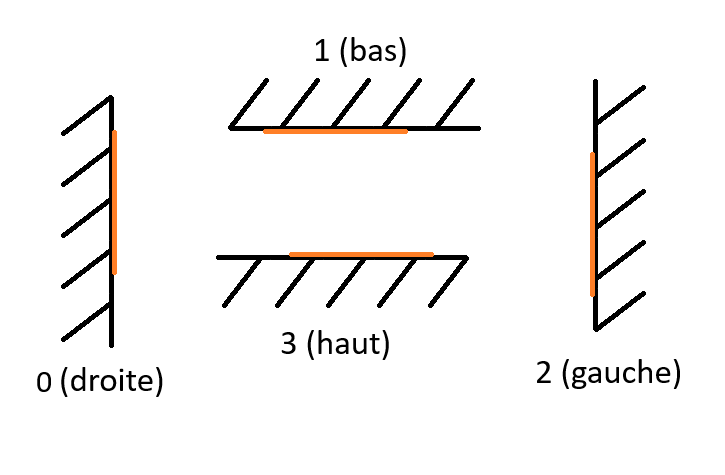
\includegraphics[width=0.7\textwidth]{images/portal1.png}
    \end{figure}
\end{frame}

\begin{frame}
    \frametitle{Les portails \\
                \small ??}
    \begin{block}{}
        
    \end{block}
    \begin{figure}
        \centering
        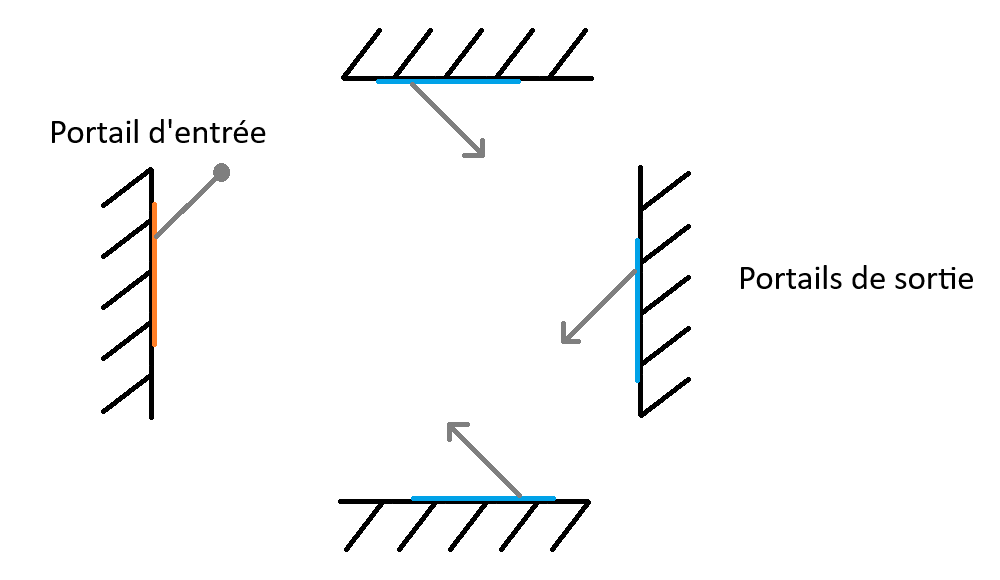
\includegraphics[width=0.7\textwidth]{images/portal2.png}
    \end{figure}
\end{frame}

\subsection{Les rendus}

\begin{frame}
    \frametitle{Les rendus}
    \begin{block}{}
        \begin{itemize}
            \item Récupération des sommets triés
            \item Envoie des rayons dans l'ordre avec DDA
        \end{itemize}
    \end{block}
    \begin{figure}
        \centering
        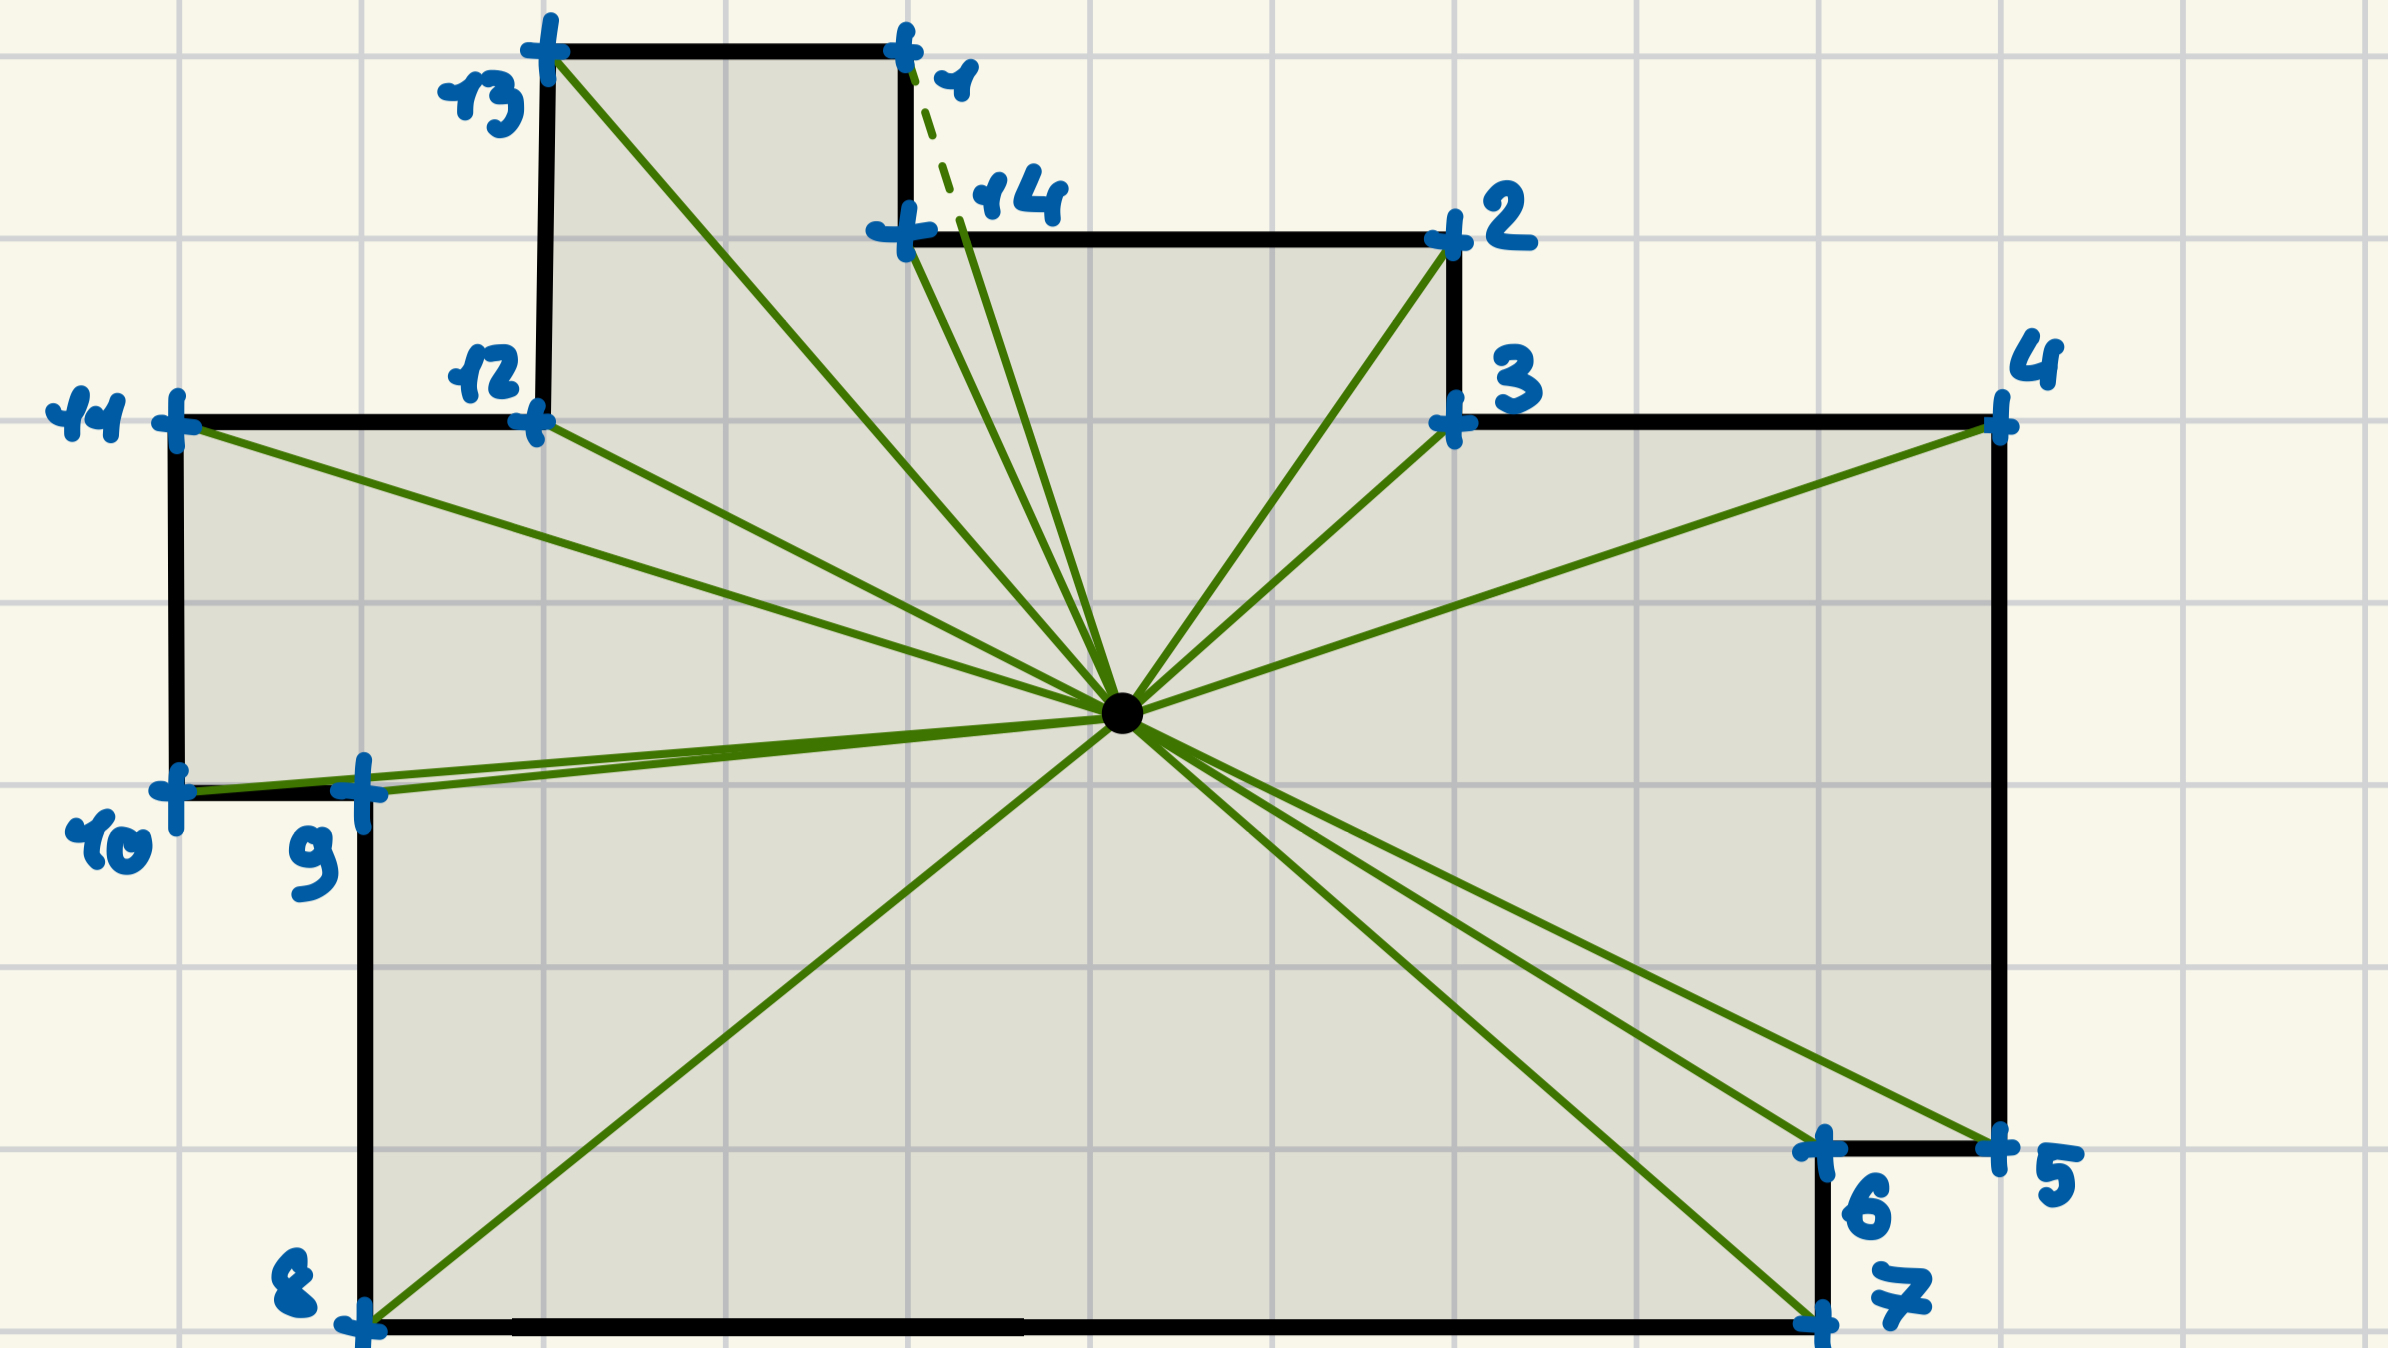
\includegraphics[width=0.7\textwidth]{images/envoie-rayon-ordre.jpeg}
    \end{figure}
\end{frame}

\begin{frame}
    \frametitle{Les rendus}
    \begin{block}{Projection des sommets}
        \begin{itemize}
            \item Déterminer la hauteur du segment (sommet en 3D) et sa position.
        \end{itemize}
    \end{block}
    \begin{figure}
        \centering
        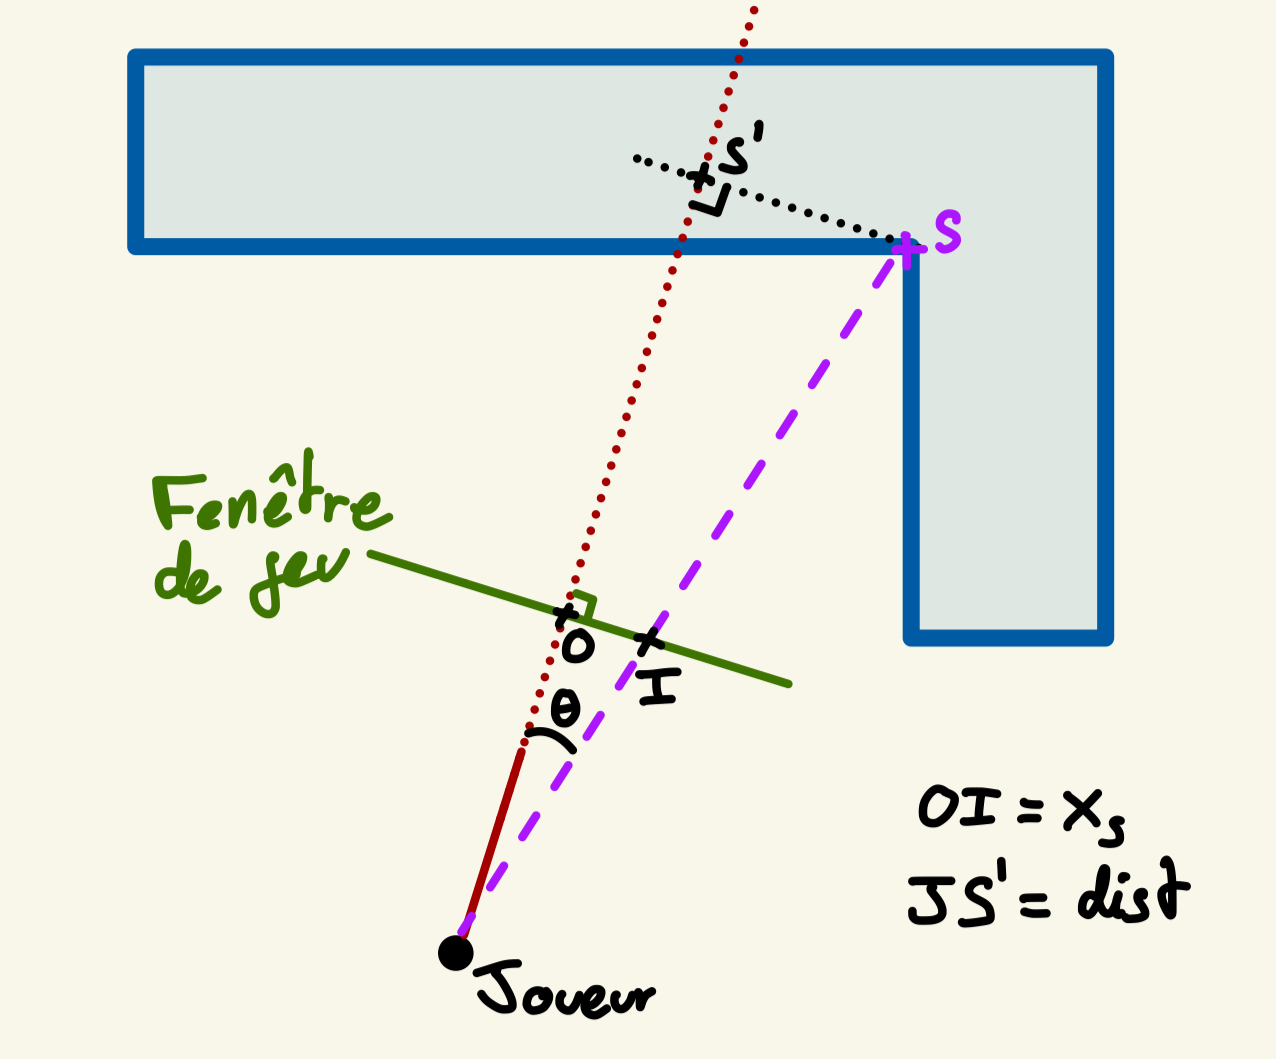
\includegraphics[width=0.7\textwidth]{images/shemaLanceRayon01.jpeg}
    \end{figure}
\end{frame}

\begin{frame}
    \frametitle{Les rendus}
    \begin{block}{}
        \begin{itemize}
            \item Résultat sans textures.
        \end{itemize}
    \end{block}
    \begin{figure}
        \centering
        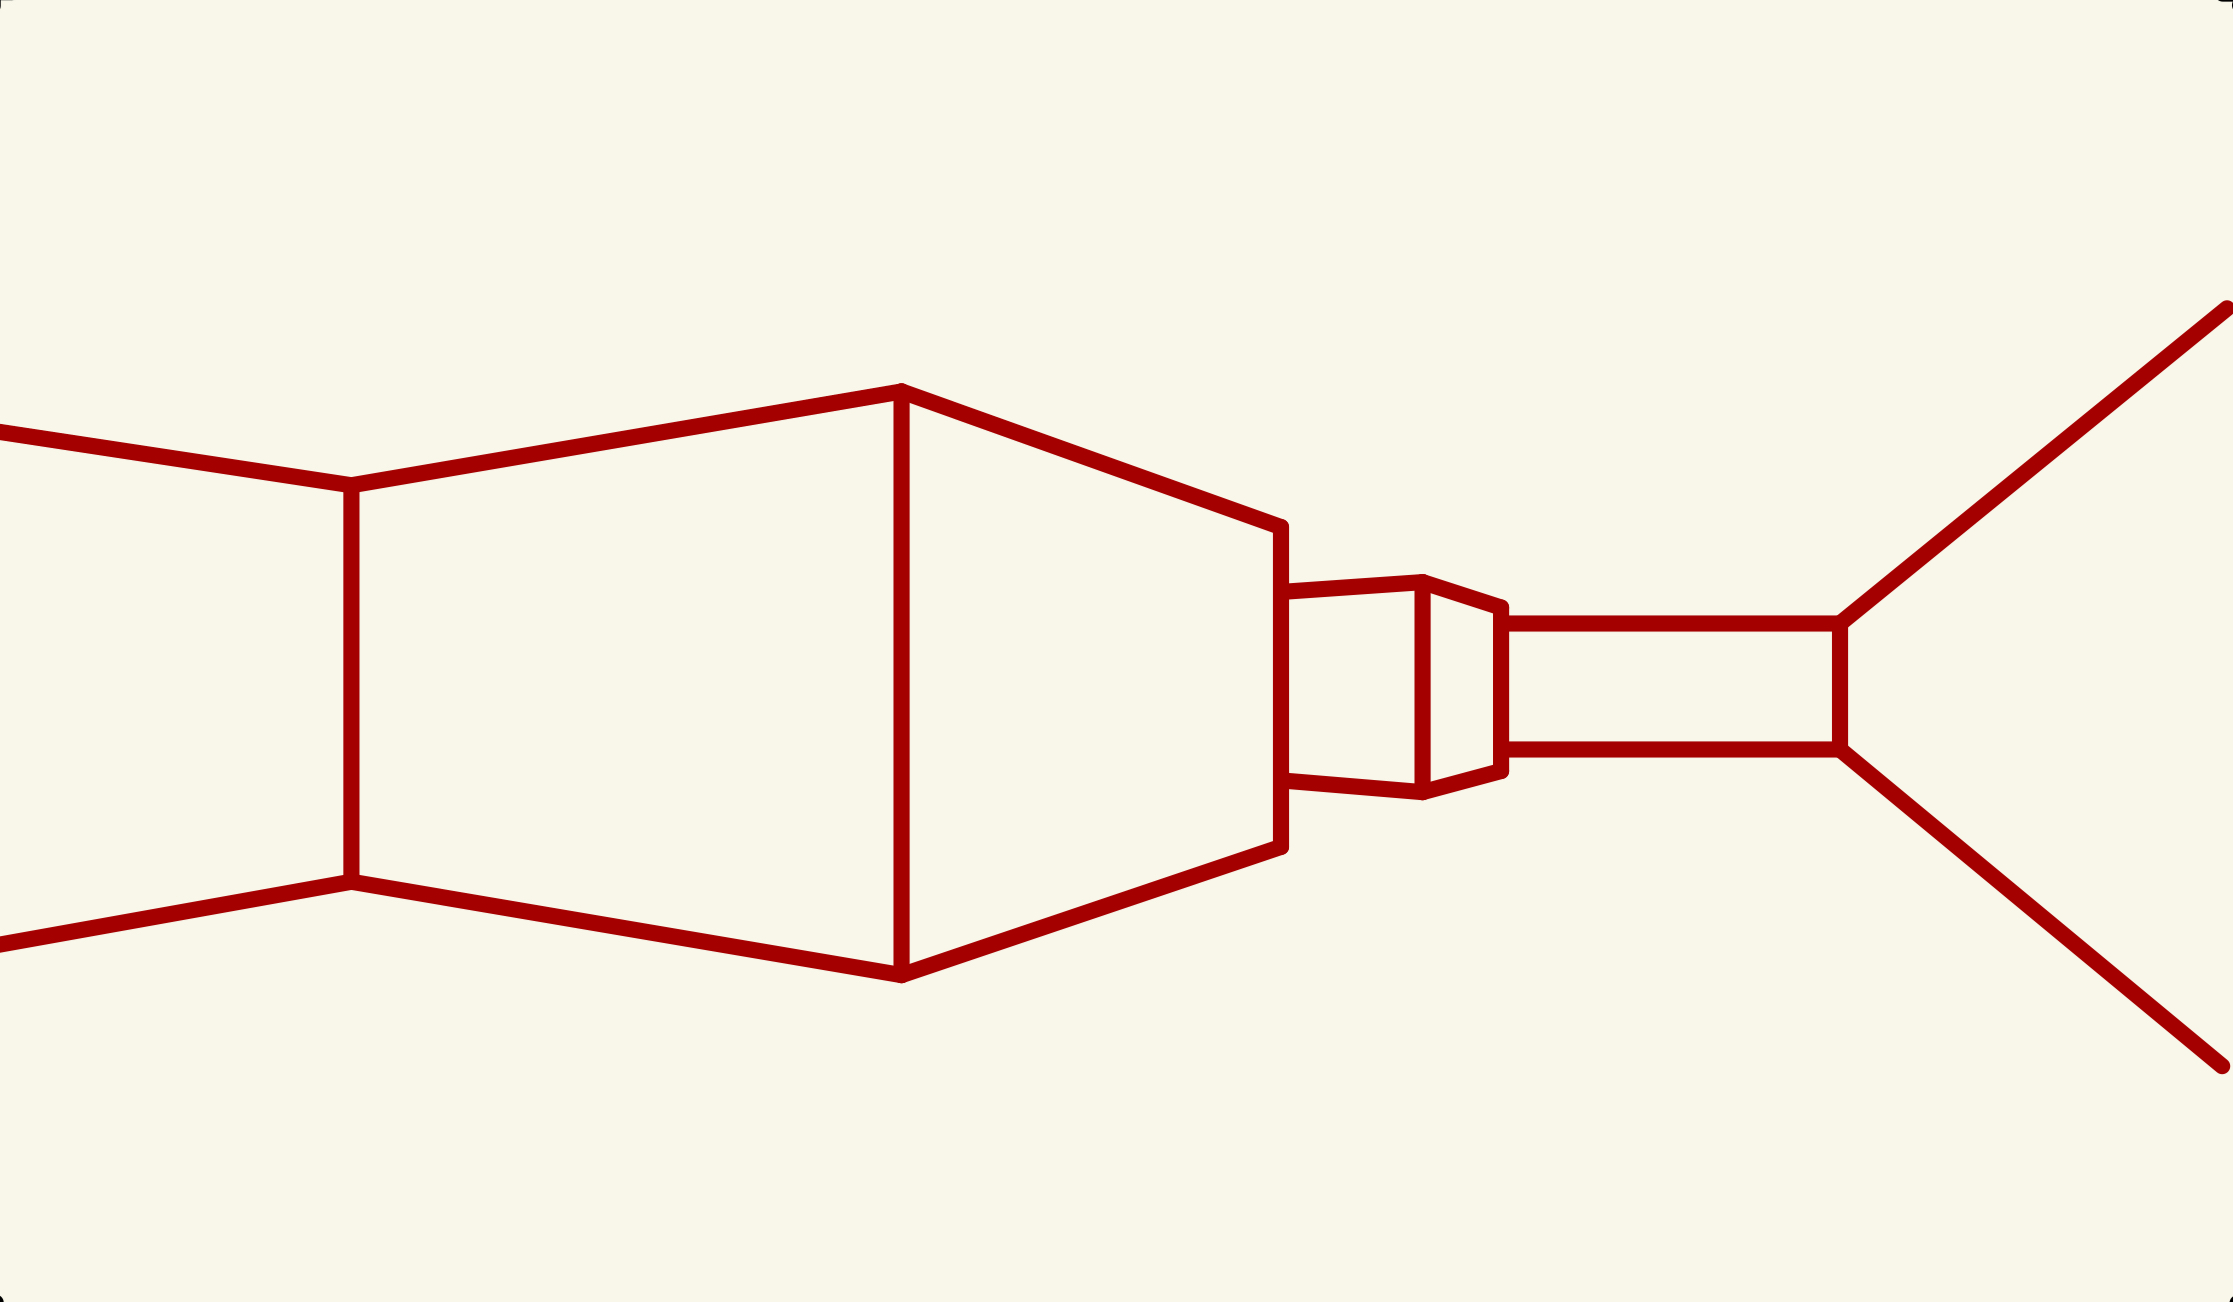
\includegraphics[width=0.7\textwidth]{images/rendu-sans-texture.jpeg}
    \end{figure}
\end{frame}

\begin{frame}
    \frametitle{Les rendus}
    \begin{block}{}
        \begin{itemize}
            \item Résultat avec textures.
        \end{itemize}
    \end{block}
    \begin{figure}
        \centering
        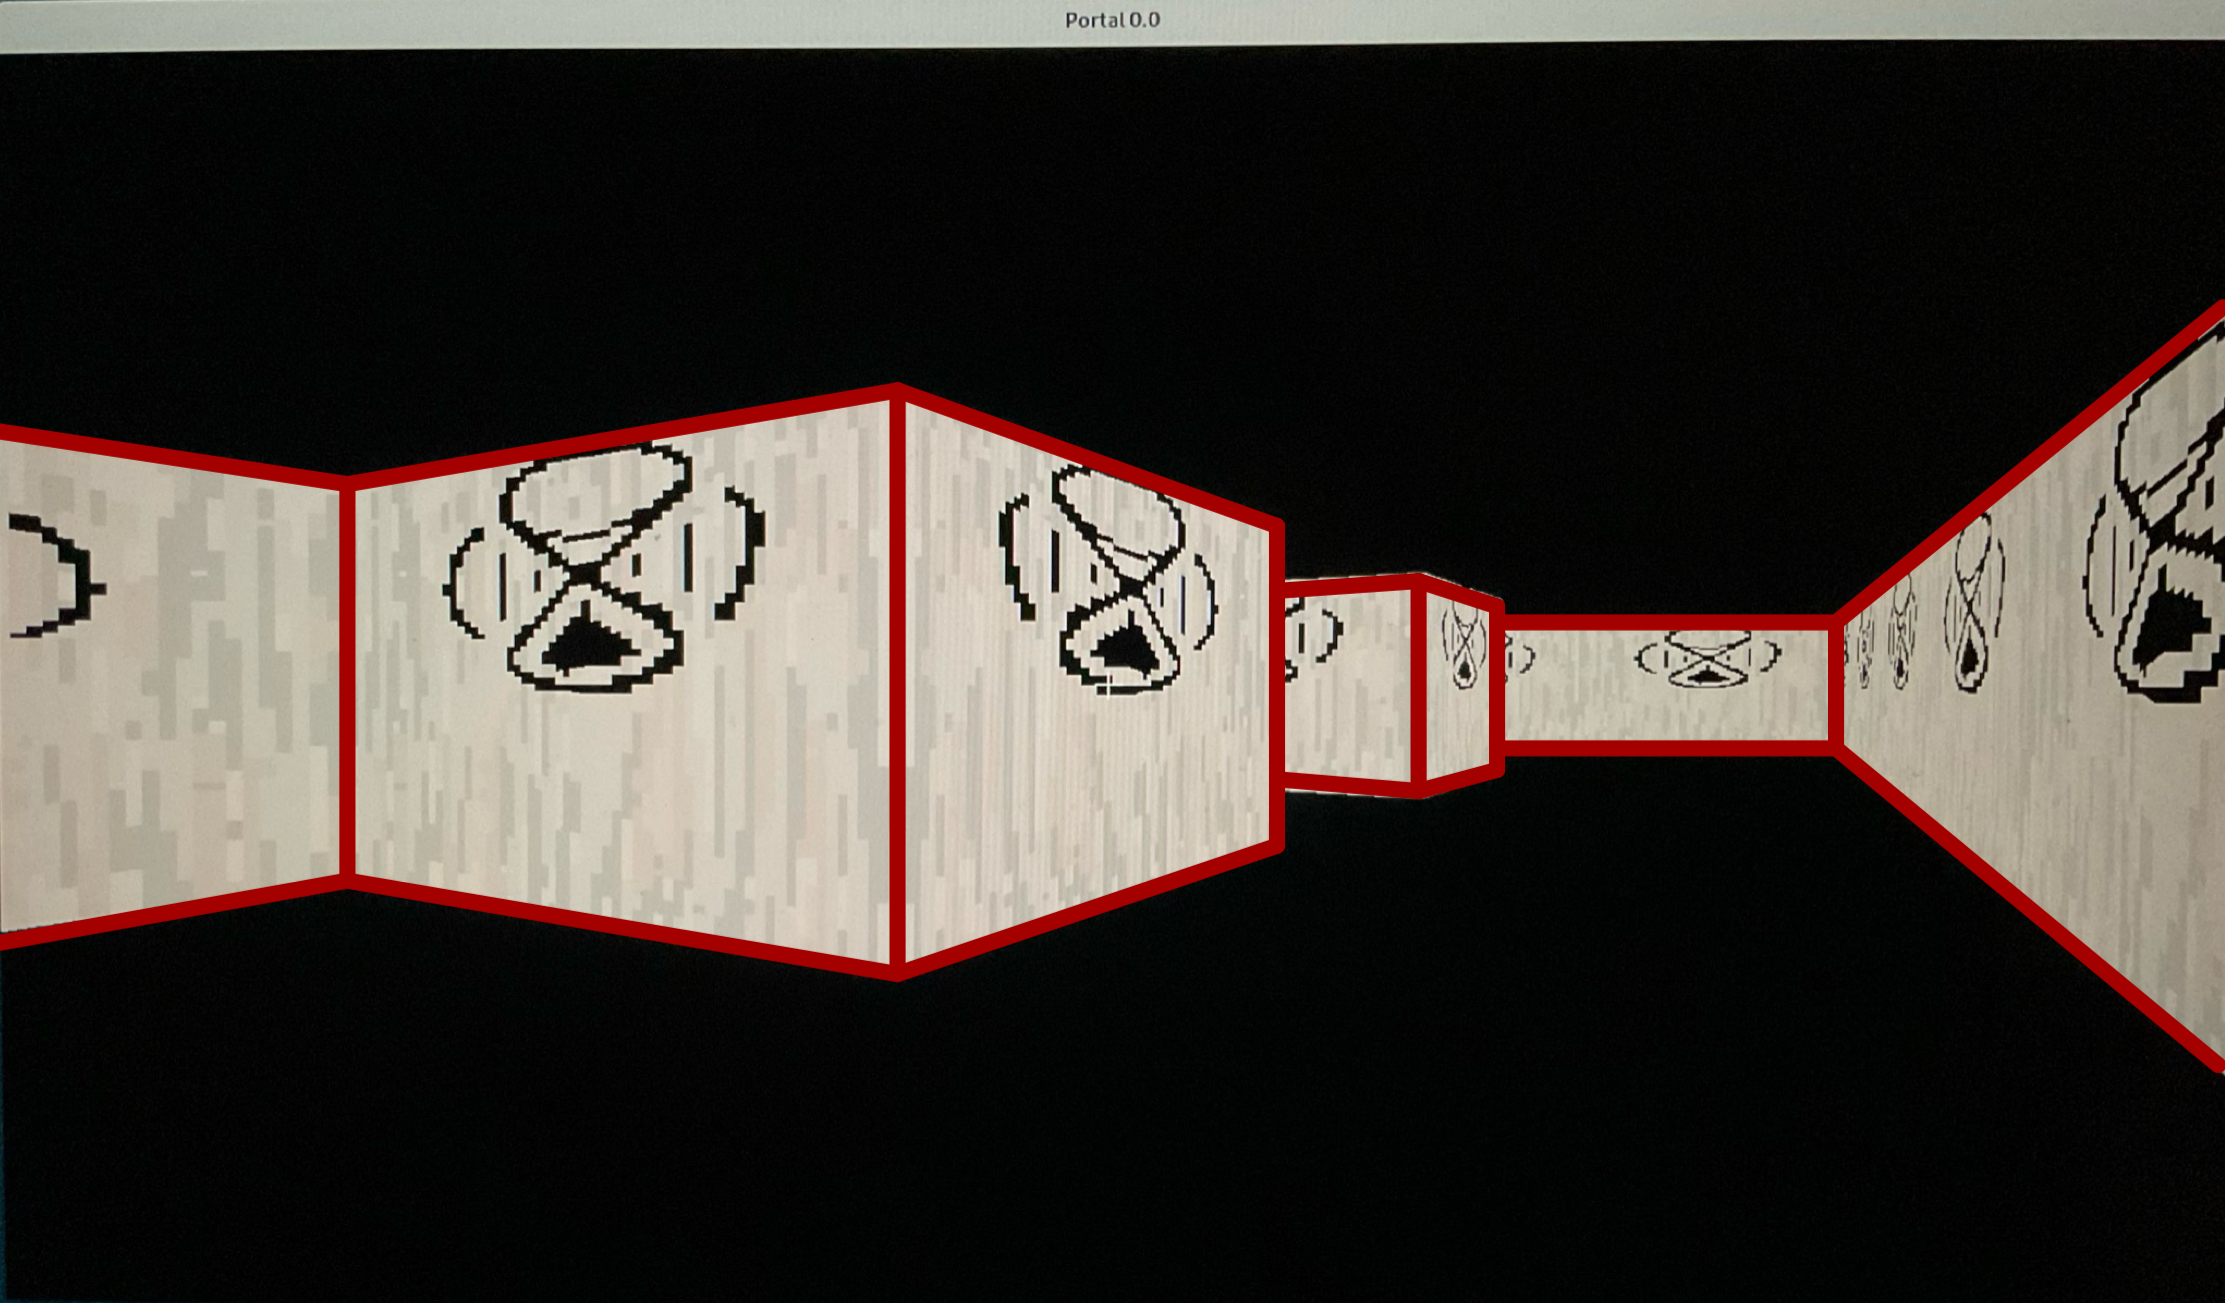
\includegraphics[width=0.7\textwidth]{images/rendu-avec-texture.jpeg}
    \end{figure}
\end{frame}

\section{Conclusion}

\begin{frame}
    \frametitle{Conclusion}
    \begin{block}{}
        \centering
        Merci de votre attention.
    \end{block}
\end{frame}

\begin{frame}
    \frametitle{Conclusion \\
                \small Remerciements}      
    \begin{block}{}
        
    \end{block}         
\end{frame}

\section*{Questions}

\begin{frame}
    \frametitle{Questions}
    \begin{block}{}
        \centering
        Avez-vous des questions ?
    \end{block}
\end{frame}

\end{document}